\documentclass[tikz,border=10pt]{standalone}
\begin{document}
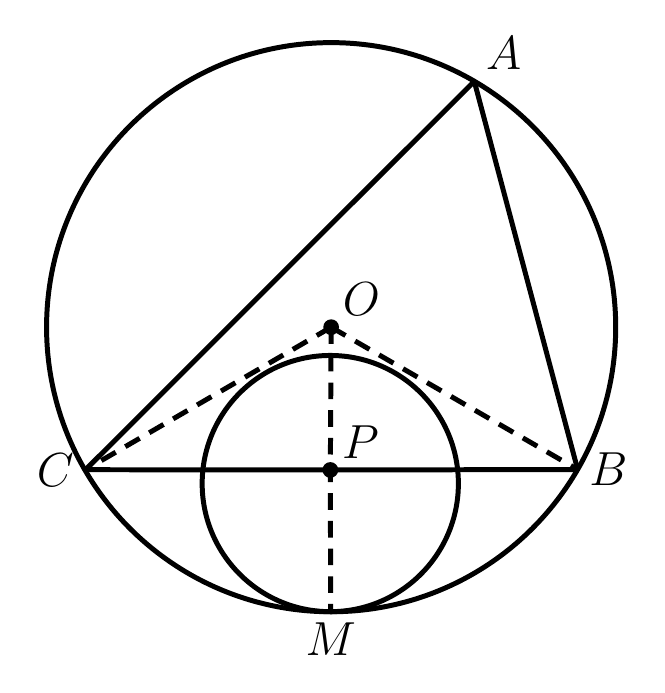
\begin{tikzpicture}[line width=1.8pt, line join=round, font=\fontsize{17}{20.4}\selectfont]
\coordinate (A) at (1.794,3.384);
\coordinate (B) at (3.107,-1.547);
\coordinate (C) at (-3.143,-1.549);
\coordinate (O) at (-0.024,0.261);
\coordinate (P) at (-0.034,-1.552);




\coordinate (M) at (-0.030,-3.350);
\coordinate (S) at (-0.035,-1.725);


\draw (O) circle[radius=3.614];
\draw (S) circle[radius=1.627];


\draw (C) -- (A) -- (B);
\draw (C) -- (P) -- (B);


\draw[dash pattern=on 6pt off 4pt] (O) -- (C);
\draw[dash pattern=on 6pt off 4pt] (O) -- (B);
\draw[dash pattern=on 6pt off 4pt] (O) -- (P) -- (M);


\fill (O) circle[radius=0.100];
\fill (P) circle[radius=0.100];


\node[above right] at (A) {$A$};
\node[right] at (B) {$B$};
\node[left] at (C) {$C$};
\node[above right] at (O) {$O$};
\node[above right] at (P) {$P$};
\node[below] at (M) {$M$};
\end{tikzpicture}
\end{document}